%----------------------------------------------------------------------------------------
%-----------------------------------Script Stuff-----------------------------------------
%----------------------------------------------------------------------------------------
% JAVASCRIPT

\lstdefinelanguage{JavaScript}{
  keywords={typeof, new, true, false, catch, function, return, null, catch, switch, var, if, in, while, do, else, case, break},
  keywordstyle=\color{blue}\bfseries,
  ndkeywords={class, export, boolean, throw, implements, import, this},
  ndkeywordstyle=\color{darkgray}\bfseries,
  identifierstyle=\color{black},
  sensitive=false,
  comment=[l]{//},
  morecomment=[s]{/*}{*/},
  commentstyle=\color{purple}\ttfamily,
  stringstyle=\color{red}\ttfamily,
  morestring=[b]',
  morestring=[b]"
}

\lstset{
   language=JavaScript,
   backgroundcolor=\color{lightgray},
   extendedchars=true,
   basicstyle=\footnotesize\ttfamily,
   showstringspaces=false,
   showspaces=false,
   numbers=left,
   numberstyle=\footnotesize,
   numbersep=9pt,
   tabsize=2,
   breaklines=true,
   showtabs=false,
   captionpos=b
}

% PYTHON 
% Python style for highlighting
\newcommand\pythonstyle{\lstset{
language=Python,
basicstyle=\ttm,
otherkeywords={self},             % Add keywords here
keywordstyle=\ttb\color{deepblue},
emph={MyClass,__init__},          % Custom highlighting
emphstyle=\ttb\color{deepred},    % Custom highlighting style
stringstyle=\color{deepgreen},
frame=tb,                         % Any extra options here
showstringspaces=false            % 
}}


% Python environment
\lstnewenvironment{python}[1][]
{
\pythonstyle
\lstset{#1}
}
{}

% Python for external files
\newcommand\pythonexternal[2][]{{
\pythonstyle
\lstinputlisting[#1]{#2}}}

% Python for inline
\newcommand\pythoninline[1]{{\pythonstyle\lstinline!#1!}}
%----------------------------------------------------------------------------------------

\chapter{Technology Review}
Over the course of the project life cycle a plethora of frameworks, tools and development applications were available for integration or use with our application. This section aims to discuss the tools and technologies that were heavily considered and those that were ultimately used, why they were chosen and what alternatives were available. 

\section{Initial Considerations}
During the discussion and planning phase goals were outlined and proposed however, how to reach the end point was still very ambiguous. For this reason a lot of time was spent considering different approaches and uncovering the benefits and drawbacks of venturing down a chosen route. This brief section will outline those initially considered approaches.
\subsection{MEAN Stack}
The MEAN Stack combines the best of JavaScript based technologies. The Stack is essentially a collection of open source components that provide a streamlined environment for building dynamic web applications. 

\paragraph{}
The MEAN Stack consists of:

\begin{description}
  \item[$\bullet$] MongoDB
  \item[$\bullet$] ExpressJS
  \item[$\bullet$] Angular
  \item[$\bullet$] Node.js
\end{description}

\paragraph{}
Perhaps the greatest attribute of the MEAN Stack for developers is that it's essentially a single language development stack, which can also be one of it's most undesirable attributes depending on the developer's JavaScript competency \cite{MEAN_STACK}. Other attributes that the development team considered attractive were the vast array of libraries and modules exposed via Node, it's speed, usability and flexible structure. 

\subsubsection{MongoDB}
MongoDB is essentially a document-oriented NoSQL database. It's mainly used for high volume data storage. MongoDB uses collections and documents in place of tables like classical relational databases would. Documents consist of key-value pairs which are the basic unit of data in MongoDB.

\paragraph{}
The database is considered to be ideal for projects that need to be scalable or deal with vast amounts of data \cite{MONGODB}. An attractive benefit MongoDB yields is its user friendly nature. If an entry is made into a collection that doesn't fit a defined schema, nothing halts and instead the entry is inserted into the collection without issue allowing the developer full control.

\subsubsection{ExpressJS}
ExpressJS, or simply Express, is a web application framework for NodeJS specialized for building web applications and APIs \cite{EXPRESS}. Express forms the backend cluster of the MEAN stack, handling all interactions between the frontend and the database, making sure data is seamlessly propagated to the user. 

\paragraph{}
Express is completely reliant on API's exposed by NodeJS, acting as a thin layer over NodeJS, allowing for streamlined routing and server development with very little coding. Serving an application with Express can be accomplished with half a dozen lines of code, making it very lightweight.

\medskip
\begin{lstlisting}[caption=Serving with Express]
const express = require('express');
const path = require('path');

/* Static path definition */
app.use(express.static(__dirname + '/dist/client'));

app.get('/*', function(req,res) {

/* Serving static files */
res.sendFile(path.join(__dirname+'/dist/client/index.html'));
});

/* Exposing a port to listen for requests on (Served with NodeJS, Discussed below!) */
app.listen(process.env.PORT || 8081);

\end{lstlisting}

\subsubsection{Angular}
Angular is a front-end framework built on top of JavaScript and developed by Google that specializes in enabling the development of single-page applications \cite{ANGULAR}. Single-page applications have become increasingly popular since their breakthrough, providing an array of benefits and advantages over the traditional multi-page web application, some of those advantages being:

\begin{enumerate}
    \item[$\bullet$] The possibility to run the developed application on almost all platforms and devices.
    \item[$\bullet$] Transference of the business logic from the server to the client.
    \item[$\bullet$] Attractive user interface that utilizes application-like UI components and aesthetically pleasing transitional animations.
    \item[$\bullet$] Can support the building of applications for offline usage or testing, easing the development experience and allowing the loading of the complete application at once.
\end{enumerate}

While the benefits listed above \cite{SPA} are some of the more attractive features of single-page applications there are of course drawbacks. The performance of single-page applications on mobile devices has been criticized and the 'all-in' approach may be an unattractive feature for larger applications, if one element of the overall page logic causes an issue it's likely the whole page will by extension will suffer.

\subsubsection{NodeJS}
NodeJS, or simply Node, considered the backbone of the MEAN stack, is an open source, cross-platform, JavaScript run-time environment that executes JavaScipt code outside of a web browser \cite{NODE}. Using asynchronous events, Node allows the processing of multiple connections simultaneously, ideal for cloud-based applications that require scalability on demand. 

\paragraph{}
Node comes with a complete integrated web server, allowing seamless application and database deployment to the cloud with the ability to support millions of simultaneous connections \cite{NODE_TWO}. Node can be weak to larger processes, while a single thread may protect against process deadlocks, on the same token large scale freezes may occur with frequent high-resource requests.

\subsubsection{Comparing MEAN and MERN}
Another technology stack that piqued the attention of the developers was the MERN Stack, which is essentially the MEAN Stack excluding Angular and including React. Research was conducted on comparing the two \cite{MEAN_STACK_vs_MERN_STACK} and the following was found:

\begin{table}[H]
\begin{tabularx}{\linewidth}{>{\parskip1ex}X@{\kern4\tabcolsep}>{\parskip1ex}X}
\toprule
\hfil\bfseries Angular
&
\hfil\bfseries React
\\\cmidrule(r{3\tabcolsep}){1-1}\cmidrule(l{-\tabcolsep}){2-2}

%% PROS, seperated by empty line or \par
\begin{compactitem}[-]
\item[+] Testing tools like Jasmine and Karma are well documented Angular frameworks that allow for seamless human-readable Unit Tests or browser/platform based test cases.
\item[+] Application logic is a lot clearer and less convoluted than React due to it's declarative nature.
\item[+] Enforces MVC-like design, giving developers an underlying structure to adhere to. React applications can be harder to maintain considering the overall design can be ambiguous and more unstructured.
\item[+] Unidirectional data flow in applications allow data to flow to more seamlessly check for a change of state.
\item[$-$] Weak ability to debug code. Debugging can be ambiguous without manual inclusion of libraries.
\end{compactitem}
\par

&

%% CONS, seperated by empty line or \par
\begin{compactitem}[-]
\item[+] Mastering React is a lot less punishing than delving into Angular, Angular being a complete framework that incorporates associated knowledge of concepts like MVC or familiarity with Typescript.
\item[+] Unidirectional data flow in applications allow data to flow to more seamlessly check for a change of state.
\item[+] Very lightweight and less cumbersome than Angular for setup and collaboration. Dependency control is managed automatically.
\item[$-$] Relies heavily on third-party libraries for actions and tasks that Angular could perform by on the fly due to it's built in service wrappers like for example Angular's built in wrappers for HTTP calls to the backend. 
\end{compactitem}

\\\bottomrule
\end{tabularx}
\caption{Advantages and Disadvantages of React \& Angular}
\end{table}

Following the comparison of both React and Angular, the team spoke both internally and at supervisory meetings about the best route to take. Conclusively, the team felt Angular had the edge over React, the main factors being:

\begin{enumerate}
    \item[$\bullet$] Jasmine and Karma were two both very attractive testing tools that the team felt would enhance the development of the project.
    \item[$\bullet$] Libraries like Angular-material and Angular-animations to name few of many are very compatible with a project of this nature, not to mention very well documented. 
    \item[$\bullet$] The team previously had exposure to Angular, which was a small bonus, however it was clear following the aforementioned research that previous trials with the framework hadn't even scraped the surface of the available features. 
\end{enumerate}

\subsection{VueJS}
VueJS is a JavaScript based framework used for building user interfaces and single page applications that can integrate seamlessly into a project at any stage. VueJS is marketed as an approachable, versatile and performant framework, boasting an incrementally adoptable system that's scaleable between a fully featured framework and a library \cite{VUE}. However a major downfall of the framework is considered to be it's steep learning curve. VueJS was trialed for two weeks by the team, and following supervisory meetings and discussions between team members, the team ultimately decided due to the steep learning curve, the intimidating documentation for beginners and lack of tutorials that it wouldn't see a place in the development stack.

\subsection{Redis}
Redis, meaning REmote DIctionary Server is an in-memory distributed key-value data-store. Redis supports multiple types of data structures including, streams, bitmaps, sets and spatial indexes to name a few \cite{REDIS_IO}. Key value databases excel at providing rapid access to information that has a corresponding function and following research and discussions with supervisors Redis was initially a very attractive inclusion into the project. The use of in-memory storage offers a number of advantages, namely data retrieval which as mentioned previously is extremely fast as well as memory writing being performed in mono-thread allows the write to be isolated, avoiding data loss \cite{REDIS}.

\paragraph{}
At early stages in the project, various machine learning implementations were being considered. Redis would have been a perfect inclusion should the project have adopted artificial intelligence in any form, allowing for rapid access and storage of short-lived large scale machine learning data.

\section{Chosen Technologies}
Following research, input from supervisors and trials of the aforementioned technologies via a developed prototype, a stack was constructed that the developers felt would fit both the objective and scope of the project. This section will outline the technologies, tools, languages, frameworks and concepts that were ultimately implemented and descriptions of relevant implementations will be illustrated at a conceptual level.

\subsection{Angular}
After the elimination of the possibility of VueJS from the prototype and the ruling out of React, Angular was the strongest contender remaining. Following trials and integration with the prototype, the team found Angular to be a very nice fit. While a stack with Flask, Python and Angular isn't traditionally common, the Angular documentation allowed for a very smooth integration \cite{ANGULAR_DOCUMENTATION}.

\paragraph{}
Within just over a week of integration into the prototype, the team were able to serve up static Angular files with Flask and establish connections and routes for accessing various defined endpoints.

\subsection{The Flask Micro-framework}
The Flask Micro-framework is designed for building simple and robust web-applications with a Python backend \cite{FLASK}. The Flask backend looks similar to a traditional Python file, functions are defined with an \textbf{@app.route()} decorator, declaring the function a handler for the endpoint which may be defined via parameters.

The performance of Flask is held in high regard when compared with frameworks of a similar nature \cite{FLASK_USAGE}. The team found Flask to be lightweight and easy to use while still yielding attractive results. Additionally, another big advantage of using Flask is having the choice of an array of Python or Flask sub-modules that enhance the functionality and development experience of working with Flask. 

\begin{python}[caption=Sample Route Definition with Flask]
@app.route('/delete/<string:_id>')
def delete(_id):
    try: 
        collection.delete_one( {'_id': ObjectId(_id) } ) 
        return redirect('/')
    except:
        return 'Error - Cant delete the object!'
\end{python}

\subsection{MongoDB Atlas}
Trialed during the development of the prototype, MongoDB Atlas proved to be worthy of inclusion into the project stack. MongoDB Atlas is a DBaaS (Database as a Service) platform designed by the same team that develops MongoDB. 

\paragraph{}
Atlas provides all the features of its database counterpart without any complexities of security or maintenance \cite{MONGO_ATLAS}. Some of these features include:

\begin{enumerate}
    \item[$\bullet$] Automated Security Features.
    \item[$\bullet$] Built-In Replication.
    \item[$\bullet$] Backups and Point-In-Time Recovery.
    \item[$\bullet$] Monitoring and Traffic Tools.
\end{enumerate}

Integration is also simplified, a URI is provided based on the development language being used that references the cluster, libraries like PyMongo allow for the dissection of the URI, providing an array of functionality relational to the URI, allowing for the interaction and control of individual collections within the cluster associated with the URI.\newline

\begin{python}[caption=Defining and Accessing a Mongo Collection with Python]
import pymongo
from pymongo import MongoClient

cluster = MongoClient("MONGO_URI")
database = cluster["example_database"]
collection = database["example_collection"]

collection.insert_one(postForCollection)
\end{python}

\section{Deployment}
An array of deployment platforms and tools for easing deployment were available to the team. Following experimentation with the prototype, a platform was decided and during development the tools to help ensure smooth deployment were identified. This section will provide a conceptual level overview of the aforementioned deployment tools and chosen platform.

\subsection{Heroku}
Heroku is an open source platform as a service cloud platform, providing extensive and well developed services for many aspects of the deployment life-cycle \cite{HEROKU}. Heroku boasts deployment simplicity, allowing the deployment of almost every type of application. Should the type of application not be supported, there are various official and third-party build-packs to allow for seamless deployment. Additionally, Heroku also supports deployment via Git, a very attractive feature considering the Version Control setup of the project.

\paragraph{}
Initially AWS had been the likely deployment platform for the application. While hands-on experience with AWS would be beneficial, the team ultimately decided to deploy the application via Heroku. Supervisory discussions and research into Heroku's different build-pack and deployment options made Heroku the clear front runner considering the nature of the developed project. The documentation is also extensive and very well written, allowing the team to save valuable time with deployment while still getting hands-on experience with a widely used cloud application platform.

\paragraph{}
Generally speaking, it's highly advantageous to employ a cloud-hosted service as an array of benefits  can be made available, these include:

\begin{enumerate}
    \item[$\bullet$] \textbf{Cost Savings} - Perhaps the biggest benefit of cloud-based services. Physical hardware investments aren't necessary, personnel isn't required to maintain hardware and the buying and management of equipment is handled via the service provider.
    \item[$\bullet$] \textbf{High Speeds} - Allowing deployment of a service in a matter of clicks, cloud computing enables the gathering of resources required for the system faster than conventional means.
    \item[$\bullet$] \textbf{Reliability} - Being one of the more attractive advantages of cloud services, reliability is measured by mainly by performance, connectivity, and security, all of which are more often than not guaranteed at a high level by cloud services .
\end{enumerate}

The aforementioned advantages \cite{CLOUD} are but a few of the more major advantages of cloud computing, though it would be disingenuous to ignore some of the disadvantages of cloud-based services which can include varying performance, potential technical issues or downtime.

\subsection{Honcho}
Honcho is a Python port of Foreman, a tool for managing procfile-based applications \cite{HONCHO}. Honcho's purpose is to abstract away any complications of the procfile format and allow the application to be either deployed directly or export it to some other process management format. Another benefit of Honcho in this context and the main reason it was employed is down to it's utility of allowing multiple processes to run in unison.

\begin{figure}[H]
    \centering
    \textbf{python: gunicorn runner:app -b 0.0.0.0:8087\\ node: npm install \&\& npm start -b 0.0.0.0:8081}
    \caption{Honcho Procfile}
    \label{image:honchoProcfile}
\end{figure}

\paragraph{}
Honcho allows a procfile to be defined (\textit{As outlined in \textbf{Fig.\ref{image:honchoProcfile}}}) in such a way that permits the specification of multiple processes to be ran on the cloud without employing additional Dyno workers, in this case, both the Python server for the API and the Express server to serve the static files can be ran in unison without any additional workers. The port must also be specified otherwise Heroku will assign a random port number to run on.

\begin{figure}[H]
    \centering
    \textbf{web: honcho -f ProcfileHoncho start}
    \caption{Heroku Procfile}
    \label{image:herokuProcfile}
\end{figure}

The Heroku procfile (\textit{As outlined in \textbf{Fig.\ref{image:herokuProcfile}}}) consists of a single line that starts the Honcho procfile, it acts as a type of necessary procfile proxy, since the contents of the Honcho procfile wouldn't run correctly in this procfile, it points Heroku to the Honcho procfile.

\begin{center}

\end{center}

\section{Languages}
Working with a diverse stack naturally means an array of languages have to be employed, especially languages that wouldn't regularly see collaboration. This section will serve as an overview of the programming languages incorporated and provide a high-level review of each.

\subsection{Python}
Python is a high-level language, allowing developers to very efficiently express large ideas and prototype out complex functionality fast. Python is suitable for programmers of any skill-level, however has a relatively steep learning curve but is still very welcoming for beginners, described as an easy to learn but hard to master programming language.

\paragraph{}
Python has become one of the most widely used languages globally in the last decade, a result of multiple factors, not limited to but including it's extensive range of libraries, detailed and straightforward documentation \cite{PYTHON} and the overall versatility of the language.

\paragraph{}

\subsection{JavaScript}
JavaScript is a high-level, just-in-time compiled multi-paradigm programming language. JavaScript uses curly-bracket syntax, first-class functions, prototype-based object-orientation and dynamic typing \cite{JAVASCRIPT}.

\paragraph{}
JavaScript is the backbone behind the creation and functionality of dynamic website content. If something moves, refreshes or otherwise changes on the screen, it's made possible with JavaScript, so naturally with the technology stack being used to develop the defined web-application, JavaScript will undoubtedly play a big role.

\subsection{TypeScript}
TypeScript is a super-set of JavaScript, as a result, JavaScript is still permitted within a TypeScript environment. TypeScript is considered a lot more developer-friendly than JavaScript, less declaration is needed and functional errors generally won't forbid compilation, making it a lot more manageable within larger systems.

\paragraph{}
One of the bigger changes TypeScript brings is the way in which it can declare variables. In JavaScript the variable is interpreted by how the developer manages and manipulates the variable, TypeScript allows for the specific declaration, for example, 'string', 'number' and 'boolean' may be unambiguously declared.

\subsection{HTML}
Hypertext Markup Language is the standard markup language for displaying documents in a web browser. Generally HTML is assisted by technologies like Cascading Style Sheets and scripting languages like the aforementioned JavaScript. Naturally, since the developed project is a web-application, HTML is prevalent throughout the frontend.

\subsection{CSS}
Cascading Style Sheets, or CSS, is a style-sheet language mainly used for the description of the presentation of a document written in a markup language, like HTML. CSS is considered a pillar technology of the web alongside HTML and JavaScript.

\paragraph{}
CSS is generally described as the 'skin' of an application or website, as it can control the scale, position and aesthetic of an overall system. CSS is considered an easy to use tool but is still very hard to master, so naturally those experienced and with an artistic eye can easy manipulate an initially dilapidated website into something a bit more aesthetically pleasing.

\section{Development Environment Tools}
This section will discuss the tools and features employed during the development cycle of the project that helped ease the overall development experience and help make it as smooth as it could be.

\subsection{Visual Studio Code}
The primary source-code editor used throughout the project was Microsoft's Visual Studio Code \cite{VS_CODE}. There were multiple reasons the team chose Visual Studio Code as the primary code editor during the project development cycle.

\subsubsection{Debugging}
Employing Python, JavaScript, TypeScript and other minor languages like HTML \& CSS in the project meant having a code editor that could support the debugging of all relevant languages would save a great deal of time and effort during the development cycle, not to mention improve the overall quality of the project by extension.

\subsubsection{Extensions}
A wide range of extensions are available for use with Visual Studio Code, these can include extensions to help with debugging, testing, or just language-specific extensions. During the development phase not only were all necessary language-specific extensions employed, but other quality-of-life extensions like the \textit{Angular Essentials} and \textit{Python Library Version Manager} extensions \cite{EXTENSIONS} were immensely beneficial.

\subsection{Postman}
Postman is a specialized tool intended to help test or dissect RESTful API's. Postman allows testing of API's via a very user-friendly user interface without the chore of writing blocks of code to test the functionality.

\paragraph{}

\begin{figure}[H]
	\caption{Postman API Requests}
	\label{image:postman}
	\centering
	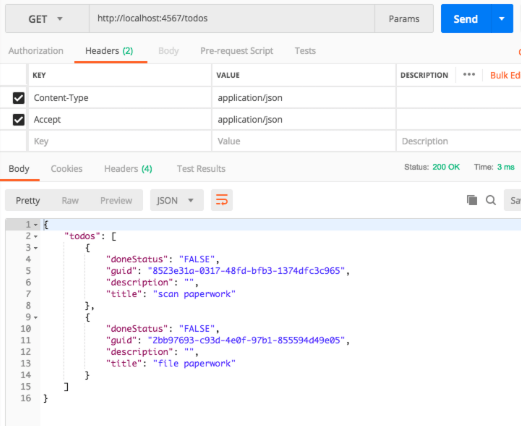
\includegraphics[width=0.8\textwidth]{images/postman.png}
\end{figure}	

Instead of writing up various tests in Flask to test each route and it's expected responses, a simple JSON body can be created with Postman and used send requests to any available endpoint. While Postman use did fade away as the project became slightly more convoluted, during the initial and prototyping stages it was very valuable.

\subsection{Ngrok}
Ngrok is a tool that can expose local servers behind network address translations and firewalls to the public internet over secure tunnels. Ngrok was very attractive, it would in theory allow the team to work off the same externally hosted server / API simultaneously, unfortunately it didn't see much use in this regard, however there were other uses the tool would be applied to.

\paragraph{}
PyNgrok, a Python module that wraps the functionality of Ngrok into an easy to use library was discovered and used during development to test deployment of the application. The API was the most troublesome cluster of the application to deploy to the cloud, Ngrok allowed the deployment of the application while having requests being directed externally to the Ngrok address, allowing the gradual deployment of the application which enabled thorough troubleshooting.

\section{Representational State Transfer}
Representational State Transfer, or simply REST, outlines a set of constraints to be used for creating Web services and is defined as a software architectural style. Services that conform to the REST architectural style are considered RESTful services. These RESTful services provide interoperability between systems over the internet \cite{REST}.

\paragraph{}
In similar fashion to HTTP, RESTful services use request methods like GET, PUT, POST, DELETE, ensuring portability. REST is stateless, meaning  every request happens in absolute isolation. When the client makes a request, it will include all necessary information required for the surver to fulfill the request. The server will never rely on information from previous requests \cite{REST_STATE}.

\section{Testing}
After defining the technology stack for the application, complimentary testing tools were researched that would enable continuous and efficient testing of the main attributes of the project.

\subsection{Karma}
Karma is a command-line unit testing tool that can spawn a web-server and run source code against test code for each browser connected. The results of each unit test against each connected browser are examined and displayed via the command-line, highlighting which browser specific tests passed or failed.

\paragraph{}
Karma also monitors all the specified files defined within the configuration file, and checks to see if any file changes. If changes are detected, it can trigger the test to re-execute by sending a signal to the testing server to inform all of the highlighted browsers to re-run the test code. Each browser re-loads the source files, executes the defined tests and reports the results back to the server.

\subsection{Jasmine}
Jasmine is a behavior driven development framework for JavaScript. Jasmine provides functions that can help with test structuring and assertions. 

\begin{lstlisting}[caption=Test Definition with Jasmine]
describe('sorting the list of users', function() {
  it('sorts in descending order by default', function() {
    var users = ['faris', 'bob', 'jeff'];
    var sorted = sortUsers(users);
    expect(sorted).toEqual(['bob', 'faris', 'jeff']);
  });
});
\end{lstlisting}

As the amount of tests grow, keeping them structured, in order and documented is vital, and Jasmine helps achieve this. The \textit{describe} function is used to group tests together while multiple individual tests, defined with the \textit{it} function can be contained within the overall describe function.